\renewcommand{\theequation}{\theenumi}
\renewcommand{\thefigure}{\theenumi}
\begin{enumerate}[label=\thesubsection.\arabic*.,ref=\thesubsection.\theenumi]
\numberwithin{equation}{enumi}
\numberwithin{figure}{enumi}

\item Find the equation to the circle which passes through the points $\myvec{ 1 \\ -2 }$ and $\myvec{ 4 \\ -3 }$ and which has its centre on the straight line $\myvec{ 3 & 4 }x = 7$.
%
\\
\solution
The equation of circle can be expressed as
\begin{align}
    \vec{x}^T\vec{x}-2\vec{C}^T\vec{x}+f = 0
\end{align}
$\vec{C}$ is the centre  and substituting the points in the equation of circle we get
\begin{align}
2\myvec{1 & -2}\vec{C}-f &= 5\\
2\myvec{4 & -3}\vec{C}-f &= 25\\
\myvec{3 & 4}\vec{C} &= 7
\end{align}
can be expressed in matrix form
\begin{align}
\myvec{3 & 4 & 0 \\
2 & -4 & -1 \\
8 & -6 & -1}
\myvec{\vec{C}\\f} = \myvec{ 7 \\ 5 \\ 25}
\end{align}

Row reducing the augmented matrix
\begin{align}
\myvec{3 & 4 & 0 & 7\\
2 & -4 & -1 & 5 \\
8 & -6 & -1 & 25}
\xleftrightarrow{R_1\leftarrow R_1/3}
\myvec{1 & \frac{4}{3} & 0 & \frac{7}{3}\\ \\
2 & -4 & -1 & 5 \\ 
8 & -6 & -1 & 25}
\end{align}

\begin{align}
\xleftrightarrow[R_3\leftarrow R_3 - 8R_1]{R_2\leftarrow R_2 - 2R_1}
\myvec{1 & \frac{4}{3} & 0 & \frac{7}{3}\\ \\
0 & \frac{-20}{3} & -1 & \frac{1}{3} \\ \\
0 & \frac{-50}{3} & -1 & \frac{19}{3}}
\end{align}

\begin{align}
\xleftrightarrow{R_2\leftarrow \frac{-3}{20}R_2 }
\myvec{1 & \frac{4}{3} & 0 & \frac{7}{3}\\ \\
0 & 1 & \frac{3}{20} & \frac{-1}{20} \\ \\
0 & \frac{-50}{3} & -1 & \frac{19}{3}}
\end{align}

\begin{align}
\xleftrightarrow{R_3\leftarrow R_3 + \frac{50}{3}R_2}
\myvec{1 & \frac{4}{3} & 0 & \frac{7}{3}\\ \\
0 & 1 & \frac{3}{20} & \frac{-1}{20} \\ \\
0 & 0 & \frac{3}{2} & \frac{11}{2}}
\end{align}
\begin{align}
\vec{C} = \myvec{\frac{47}{15}  \\ \\ \frac{-3}{5} }
f = \frac{11}{3}
\end{align}
\begin{align}
f = \frac{11}{3}
\end{align}
The required circle equation,
\begin{align}
\vec{x}^T\vec{x}-2\myvec{\frac{47}{15} & \frac{-3}{5} }\vec{x} + \frac{11}{3} = 0
\end{align}

\begin{figure}[!ht]
\centering
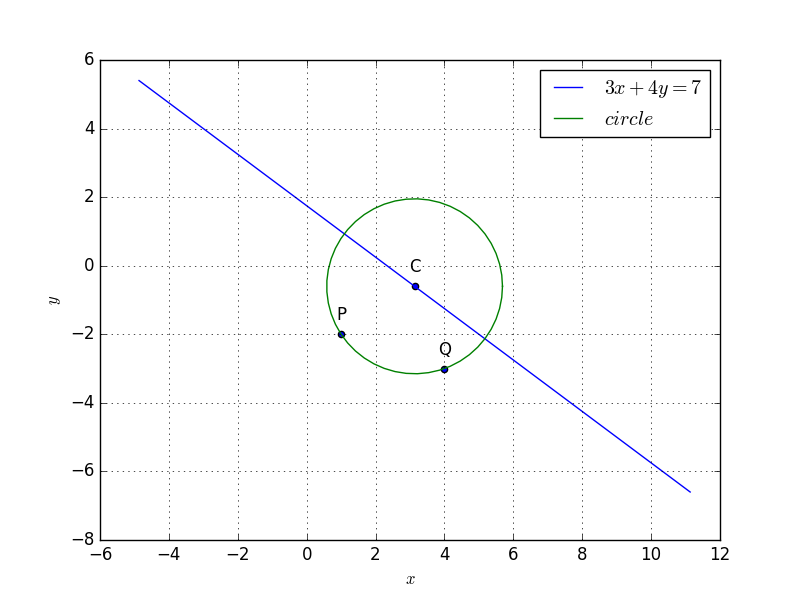
\includegraphics[width=\columnwidth]{./solutions/17/13/figure.png}
\caption{Circle passing through point P and Q also centre lie on the line 3x+4y=7}
\label{eq:solutions/17/13/Fig}
\end{figure}

Find the equation to the circle that passes through the points:
\begin{align}
\vec{x_1} = \myvec{1\\2},\vec{x_2} = \myvec{3\\-4} , \vec{x_3} = \myvec{5\\-6}
\end{align}
\solution
The equation of circle in vector form is given by:
\begin{align}
\vec{x^Tx}+2\vec{x^Tu}+f = 0 \label{eq:solutions/17/16/eq:1}
\end{align}
Using $\vec{x_1}, \vec{x_2}, \vec{x_3}$ in \eqref{eq:solutions/17/16/eq:1},
\begin{align}
\vec{x_1}^T\vec{x_1}+2\vec{x_1}^T\vec{u}+f=0\\
\vec{x_2}^T\vec{x_2}+2\vec{x_2}^T\vec{u}+f=0\\
\vec{x_3}^T\vec{x_3}+2\vec{x_3}^T\vec{u}+f=0
\end{align}
The above system can be written in matrix form as:
\begin{align}
\myvec{2\vec{x_1}^T & 1\\2\vec{x_2}^T & 1\\2\vec{x_3}^T & 1}\myvec{\vec{u}\\f}=\myvec{-\vec{x_1}^T\vec{x_1}\\-\vec{x_1}^T\vec{x_1}\\-\vec{x_3}^T\vec{x_3}} \label{eq:solutions/17/16/eq:2}
\end{align}
Substituting the values for $\vec{x_1}, \vec{x_2}, \vec{x_3}$ in \eqref{eq:solutions/17/16/eq:2},
\begin{align}
\myvec{2 & 4 & 1\\6 & -8 & 1\\10 & -12 & 1}\myvec{\vec{u}\\f}&=\myvec{-5\\-25\\-61} \label{eq:solutions/17/16/eq:3}
\end{align}
Using row echelon form to reduce \eqref{eq:solutions/17/16/eq:3}, we get:
\begin{align}
\xleftrightarrow[R_3\rightarrow R_3-5R_1]{R_2\rightarrow R_2-3R_1}\myvec{2 & 4 & 1 & -5\\0 & -20 & -2 & -10\\ 0 & -32 & -4 & -36}\\
\xleftrightarrow[R_3\rightarrow -\frac{1}{4}R_3]{R_2 \rightarrow -\frac{1}{2}R_2}\myvec{2 & 4 & 1 & -5\\0 & 10 & 1 & 5\\ 0 & 8 & 1 & 9}\\
\xleftrightarrow[]{R_3 \rightarrow 5R_3-4R_2}\myvec{2 & 4 & 1 & -5\\0 & 10 & 1 & 5\\ 0 & 0 & 1 & 25}\\ \label{eq:solutions/17/16/eq:4}
\xleftrightarrow[R_2 \rightarrow \frac{1}{10}R_2]{R_1 \rightarrow \frac{1}{2}R_1}\myvec{1 & 2 & \frac{1}{2} & -\frac{5}{2}\\[0.2cm]0 & 1 & \frac{1}{10} & \frac{2}{5}\\[0.2cm] 0 & 0 & 1 & 25}
\end{align}
Back solving the system using \eqref{eq:solutions/17/16/eq:2} and \eqref{eq:solutions/17/16/eq:4}, we get:
\begin{align}
\myvec{\vec{u}\\f}=\myvec{-11 \\ -2 \\ 25} \\
\implies \vec{u} = \myvec{-11 \\ -2}, f = 25
\end{align}
The equation of the circle that passes through the points $\vec{x_1}, \vec{x_2}, \vec{x_3}$ is given by:
\begin{align}
\vec{x^Tx}+2\myvec{-11 \\ -2}^T\vec{x}+f = 0 \\
\implies x^2 + y^2 - 22x -4y + 25 = 0
\end{align}
The plot of the circle is given below:
\begin{figure}[t]
\centering
    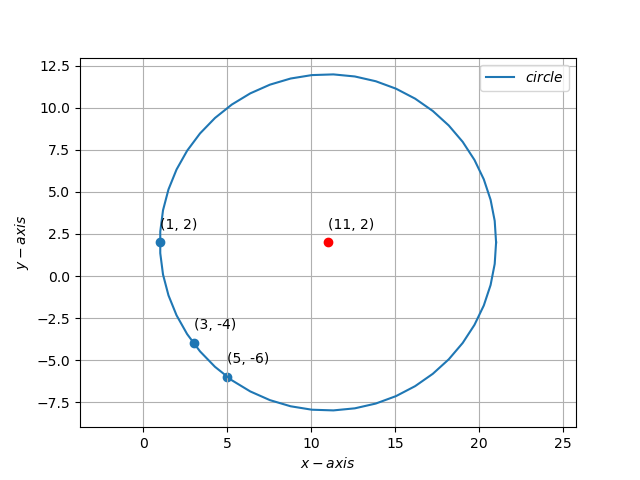
\includegraphics[width=\columnwidth]{solutions/17/16/Latex/Figure_1.png}
    \caption{Circle centered at $(11, 2)$ with radius $10$.}
    \label{eq:solutions/17/16/fig:1}
\end{figure}


\item Find the equation of circle passing through the points
\begin{align}
    \vec{x_1}=\myvec{1\\1}, \vec{x_2}=\myvec{2\\-1}, \vec{x_3}=\myvec{8\\2}\label{eq:solutions/17/17/eq:0}
\end{align}
%
\\
\solution
Vector form of the equation of circle is :
\begin{align}
\vec{x}^T\vec{x}+2\vec{x}^T\vec{u}+f=0\label{eq:solutions/17/17/eq:1}
\end{align}
For $\vec{x_1}$, $\vec{x_2}$ and $\vec{x_3}$ equation \eqref{eq:solutions/17/17/eq:1} can be written as:
\begin{align}
\vec{x_1}^T\vec{x_1}+2\vec{x_1}^T\vec{u}+f=0\\
\vec{x_2}^T\vec{x_2}+2\vec{x_2}^T\vec{u}+f=0\\
\vec{x_3}^T\vec{x_3}+2\vec{x_3}^T\vec{u}+f=0
\end{align}
In matrix form this can be written as :
\begin{align}
    \myvec{2\vec{x_1}^T&1\\2\vec{x_2}^T&1\\2\vec{x_3}^T&1}\myvec{\vec{u}\\f}&=\myvec{-\vec{x_1}^T\vec{x_1}\\-\vec{x_1}^T\vec{x_1}\\-\vec{x_3}^T\vec{x_3}}\label{eq:solutions/17/17/eq:5}
\end{align}
By putting the values of $\vec{x_1},\vec{x_2}$ and $\vec{x_3}$ from \eqref{eq:solutions/17/17/eq:0} in \eqref{eq:solutions/17/17/eq:5} we get :   
\begin{align}
 \myvec{2&2&1\\4&-2&1\\16&4&1}\myvec{\vec{u}\\f}&=\myvec{-2\\-5\\-68} \label{eq:solutions/17/17/eq:6}
\end{align}
Using Gaussian Elimination method :
\begin{align}
\xleftrightarrow[R_2 \leftarrow R_2-4R_1]{R_1 \leftarrow \frac{1}{2}R_1}\myvec{1&1&\frac{1}{2}&-1\\0&-6&-1&-1\\16&4&1&-68}\\
\xleftrightarrow{R_3 \leftarrow R_3-16R_1}\myvec{1&1&\frac{1}{2}&-1\\0&-6&-1&-1\\0&-12&-7&-52}\\
\xleftrightarrow[R_3 \leftarrow R_3+124R_2]{R_2 \leftarrow -\frac{1}{6}R_2}\myvec{1&1&\frac{1}{2}&-1\\[0.2cm]0&1&\frac{1}{6}&\frac{1}{6}\\[0.2cm]0&0&-5&-50}\label{eq:solutions/17/17/eq:9}
\end{align}
Using \eqref{eq:solutions/17/17/eq:6} and \eqref{eq:solutions/17/17/eq:9} we get : 
\begin{align}
\myvec{\vec{u}\\f}&=\myvec{-\frac{9}{2}\\[0.1cm]-\frac{3}{2}\\[0.1cm]10}\\
\vec{u}&=\myvec{-\frac{9}{2}\\[0.1cm]-\frac{3}{2}}\\
f&=10   
\end{align}
By putting the values of $\vec{u}$ and f in \eqref{eq:solutions/17/17/eq:1} we get : 
\begin{align}
\vec{x}^T\vec{x}+2\myvec{-\frac{9}{2}\\[0.1cm]-\frac{3}{2}}^T\vec{x}+10&=0\label{eq:solutions/17/17/eq:14}\\
x^2+y^2-9x-6y+10&=0\label{eq:solutions/17/17/eq:15}
\end{align}
Plot of the circle given by equation \eqref{eq:solutions/17/17/eq:15} is as follows :
\begin{figure}[h]
\centering
    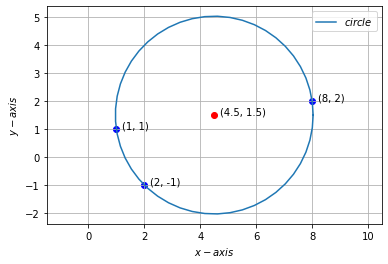
\includegraphics[width=\columnwidth]{solutions/17/17/circle3.png}
    \caption{A circle centered at $(4.5, 1.5)$ with radius $3.53$.}
    \label{eq:solutions/17/17/circle}
\end{figure}


\end{enumerate}
